\section{Systematic uncertainties}
\label{sec:systematics}
The source of systematic uncertainties of our \gammaiso--hadron measurement are the following:
\begin{itemize}
    \item Purity\\
The uncertainty of the purity measurement, which is described in Section~\ref{sec:puritysystematics}, is propagated to the correlation function measurement following Equation~\ref{eq:FinalSubtraction}. The resulting uncertainty on the correlation function is a relative $\pm18\%$ for pp data and  $\pm12\%$ for \pPb~data . As described in Section~\ref{sec:puritysystematics}, a large fraction of the purity total uncertainty is either statistical uncertainty or systematic uncertainties that arise due to limited data sample. Therefore, the purity uncertainty in pp and \pPb~data are largely uncorrelated. As a conservative approach, we take them to be totally uncorrelated.

\item	Underlying Event:\\
As described in Section~\ref{sec:UEsubtraction}, the uncertainty of the UE subtraction originates from statistical fluctuations in the ZYAM estimate. It propagates directly to our per-trigger yields. It ranges from 7\% to 15\% depending on the \zt~bin and data. This uncertainty is fully correlated in $\varphi$ for a given \zt~bin, but totally uncorrelated among \zt~bins, and totally uncorrelated between pp and \pPb~datasets.

\item Tracking performance :\\
To estimate the systematic uncertainty of our charged-particle $\pt$ measurement with ITS-only track reconstruction, we perform MC simulation studies and make a comparison with published \pt~spectra that used the ALICE standard tracking (i.e. including TPC) in pp and \pPb~collisions at 5 TeV~\cite{Acharya:2018qsh}. As described in Section~\ref{sec:tracking}, the combined uncertainty due to track efficiency, fake rate, and bin-to-bin migration corrections amounts to $\pm5\%$ added in quadrature with the total systematic uncertainty of our reference $\pt$ spectra, which ranges from a relative 1.6 (2.1$\%$) to 1.9$\%$ (2.5$\%$) in the range $0.5<\pt<10$ \GeVc~for pp (\pPb) collisions~\cite{Acharya:2018qsh}. 

Systematic uncertainties due to secondary-particle contamination and from modelling of the particle-type composition in MC simulations are small ($<2\%$) for the range $0.5<\pt<10$ \GeVc. These were already estimated in Ref.\cite{Acharya:2018qsh} for pp and \pPb~data sets and already included in the systematic uncertainty estimate described above. 

The tracking performance between pp and \pPb~datasets is very similar, but as a conservative approach we take the systematic uncertainties to be completely uncorrelated.



\item Acceptance mismatch due to boost:\\
As described in Section~\ref{sec:bootstudy}, our \textsc{Pythia8} study of \gammaiso--hadron correlations show that the impact of an acceptance mismatch between pp and \pPb~data that arises from the boost of $\Delta y = 0.47$ amounts to about $5\%$ effect irrespective of $\zt$. This estimate is subject to PDF uncertainties, which are the ones that dictate the shape of the differential cross-section of photons and associated hadrons in pseudorapidity. We chose to not apply any correction for this effect, and assign a $\pm$5$\%$ systematic uncertainty on the per-trigger hadron yields. This systematic uncertainty is taken to be completely correlated with \zt. We assign this systematic uncertainty to our \pPb~measurements only. 


\item Luminosity, trigger, photon, and vertex reconstruction:\\
Our observable is normalized per measured photon. Therefore the uncertainties related to overall normalization of the \gammaiso~\pt~spectra (such as luminosity scale, vertexing efficiency, trigger efficiency and photon reconstruction efficiency) cancel completely. Consequently, we do not assign any systematic uncertainty associated with these sources in our measurement. 
\item Photon energy scale, resolution and material budget:\\
While we are by construction totally insensitive to overall normalization, we are in principle sensitive to bin-migration or scale uncertainties that affect the shape of the photon \pt~spectra. This potential systematic uncertainty is reduced because we integrate over large photon \pt~range (12--40 \GeVc). Moreover, the EMCaL performance is such that these effects are small; for a 12 GeV cluster the resolution  $\sigma_{E}/E = 4.8\%/E\otimes 11.3\%/\sqrt{E}\otimes 1.7\%$ yields $\sigma_{E}/E =3.6\%$, and at 40 GeV this yields $\sigma_{E}/E =2.4\%$. The EMCal energy scale has been studied with beam-test data~\cite{Allen:2009aa} and comparison of $\pi^{0}\to\gamma\gamma$ events in data and simulation~\cite{Adam:2016khe}, and has an associated uncertainty if 0.8$\%$. 

The uncertainties due to photon energy scale, resolution, and material budget have been estimated for the isolated photon cross-section measurement with 7 TeV pp and 5 TeV \pPb~data and are less than 3$\%$ in the \pt~range covered in this analysis~\cite{Erwann,Acharya:2019jkx}. The effects on the per-trigger correlation functions would be even smaller. Given that this level of uncertainty are much smaller than other sources of systematic uncertainties for our measurement, we neglect them. 
\end{itemize}

Table~\ref{tab:BigSummarySystematics} presents as summary of all uncertainty estimates for our \gammaiso--hadron correlation measurement. Table~\ref{tab:pPb_FF_Uncertainties} shows the uncertainty in the \pPb~to pp ratio. 


\begin{table}
   \centering
   \caption{Summary of uncertainties in $\gammaiso$-hadron correlations, which are reported as per-trigger yields of correlated hadrons. The uncertainties quoted are relative. The ranges shown encompass the relative uncertainties for hadron \zt~in 2 ranges: Low (0.06--0.18) and High (0.18--0.6) \zt.} 
   \begin{tabular*}{1.0\columnwidth}{@{\extracolsep{\fill}}lcccc@{}}
    \hline
     & Low \zt~pp data & High~\zt~pp data & Low \zt~\pPb~data & High~\zt~\pPb~data \\
  \hline
  Statistical Uncertainty & 19\%-40\% & 30\%-49\% & 16\%-23\% & 29\%-39\% \\
  \hline 
  Photon Purity  &   18\%     & 18\% &   12\%     & 12\% \\
  Underlying Event & 8\%-15\% & 7\%-12\% & 7\%-10\% & 9\%-9\% \\
  Tracking performance &  5.6\% & 5.6\% &  5.6\% & 5.6\% \\
  Acceptance mismatch &-- & -- &5\% & 5\% \\ 
  Photon Energy Scale & $<$1\% & $<$1\%  & $<$1\% & $<$1\%\\
  Photon Energy Resolution & $<$1\% & $<$1\%  & $<$1\% & $<$1\%\\
  Material budget & $<$1\% & $<$1\% & $<$1\% & $<$1\% \\
  Luminosity scale & -- & -- & -- & -- \\
  Vertex efficiency & -- & -- & -- & -- \\ 
  Trigger corrections & -- & -- & -- & -- \\
  Photon reconstruction efficiency & -- & -- & -- & -- \\
  \hline
  Total Systematic Uncertainty & 21\%-24\% & 20\%-22\% & 15\%-16\% & 16\%-16\% \\
  \hline
  Total Uncertainty & 28\%-47\% & 34\%-54\% & 22\%-28\% & 31\%-47\% \\
  \hline
  \end{tabular*}
   \label{tab:BigSummarySystematics}
\end{table}



% 13f without new 13f_new_reconstruct data %

% \begin{table}
%   \centering
%   \caption{Summary of uncertainties in $\gammaiso$-hadron correlations, which are reported as per-trigger yields of correlated hadrons. The uncertainties quoted are relative. The ranges shown encompass the relative uncertainties for hadron \zt~in 2 ranges: Low (0.06--0.18) and High (0.18--0.6) \zt.} 
%   \begin{tabular*}{1.0\columnwidth}{@{\extracolsep{\fill}}lcccc@{}}
%     \hline
%      & Low \zt~pp data & High~\zt~pp data & Low \zt~\pPb~data & High~\zt~\pPb~data \\
%   \hline
%   Statistical Uncertainty & 19--40\% & 28--49\% & 16--24\% & 34--51\% \\
%   \hline 
%   Photon Purity  &   18\%     & 18\% &   12\%     & 12\% \\
%   Underlying Event & 8--15\% & 7--12\% & 7--10\% & 10--11\% \\
%   Tracking performance &  5.6\% & 5.6\% &  5.6\% & 5.6\% \\
%   Acceptance mismatch &-- & -- &5\% & 5\% \\ 
%   Photon Energy Scale & $<$1\% & $<$1\%  & $<$1\% & $<$1\%\\
%   Photon Energy Resolution & $<$1\% & $<$1\%  & $<$1\% & $<$1\%\\
%   Material budget & $<$1\% & $<$1\% & $<$1\% & $<$1\% \\
%   Luminosity scale & -- & -- & -- & -- \\
%   Vertex efficiency & -- & -- & -- & -- \\ 
%   Trigger corrections & -- & -- & -- & -- \\
%   Photon reconstruction efficiency & -- & -- & -- & -- \\
%   \hline
%   Total Systematic Uncertainty: & 21--24\% & 20--22\% & 15--17\% & 16--17\% \\
%   \hline
%   Total Uncertainty: & 28--47\% & 34--54\% & 22--29\% & 38--54\% \\
%   \hline
%   \end{tabular*}
%   \label{tab:BigSummarySystematics}
% \end{table}

\begin{table}[h]
\centering
\caption{Summary of leading relative uncertainties on the fragmentation ratio between proton-lead and proton-proton collisions.}
   \begin{tabular*}{1.0\columnwidth}{@{\extracolsep{\fill}}lccccc@{}}
    \hline
$\zt$ interval  & Statistical  & UE Estimate  & $\gammaiso$ Purity   & Tracking corrections & Acceptance mismatch \\
\hline
0.06--0.08 & 35\% & 15\% & 22\% & 8\% & 5\%\\
0.08--0.11 & 25\% & 11\% & 22\% & 8\% & 5\%\\
0.11--0.14 & 33\% & 13\% & 22\% & 8\% & 5\%\\
0.14--0.19 & 43\% & 16\% & 22\% & 8\% & 5\%\\
0.19--0.25 & 31\% & 11\% & 22\% & 8\% & 5\%\\
0.25--0.34 & 50\% & 15\% & 22\% & 8\% & 5\%\\
0.34--0.45 & 44\% & 11\% & 22\% & 8\% & 5\%\\
0.45--0.60 & 66\% & 15\% & 22\% & 8\% & 5\%\\
       \hline 
   \end{tabular*}
   \label{tab:pPb_FF_Uncertainties}
\end{table}




%\begin{figure}[h]
%\center
%	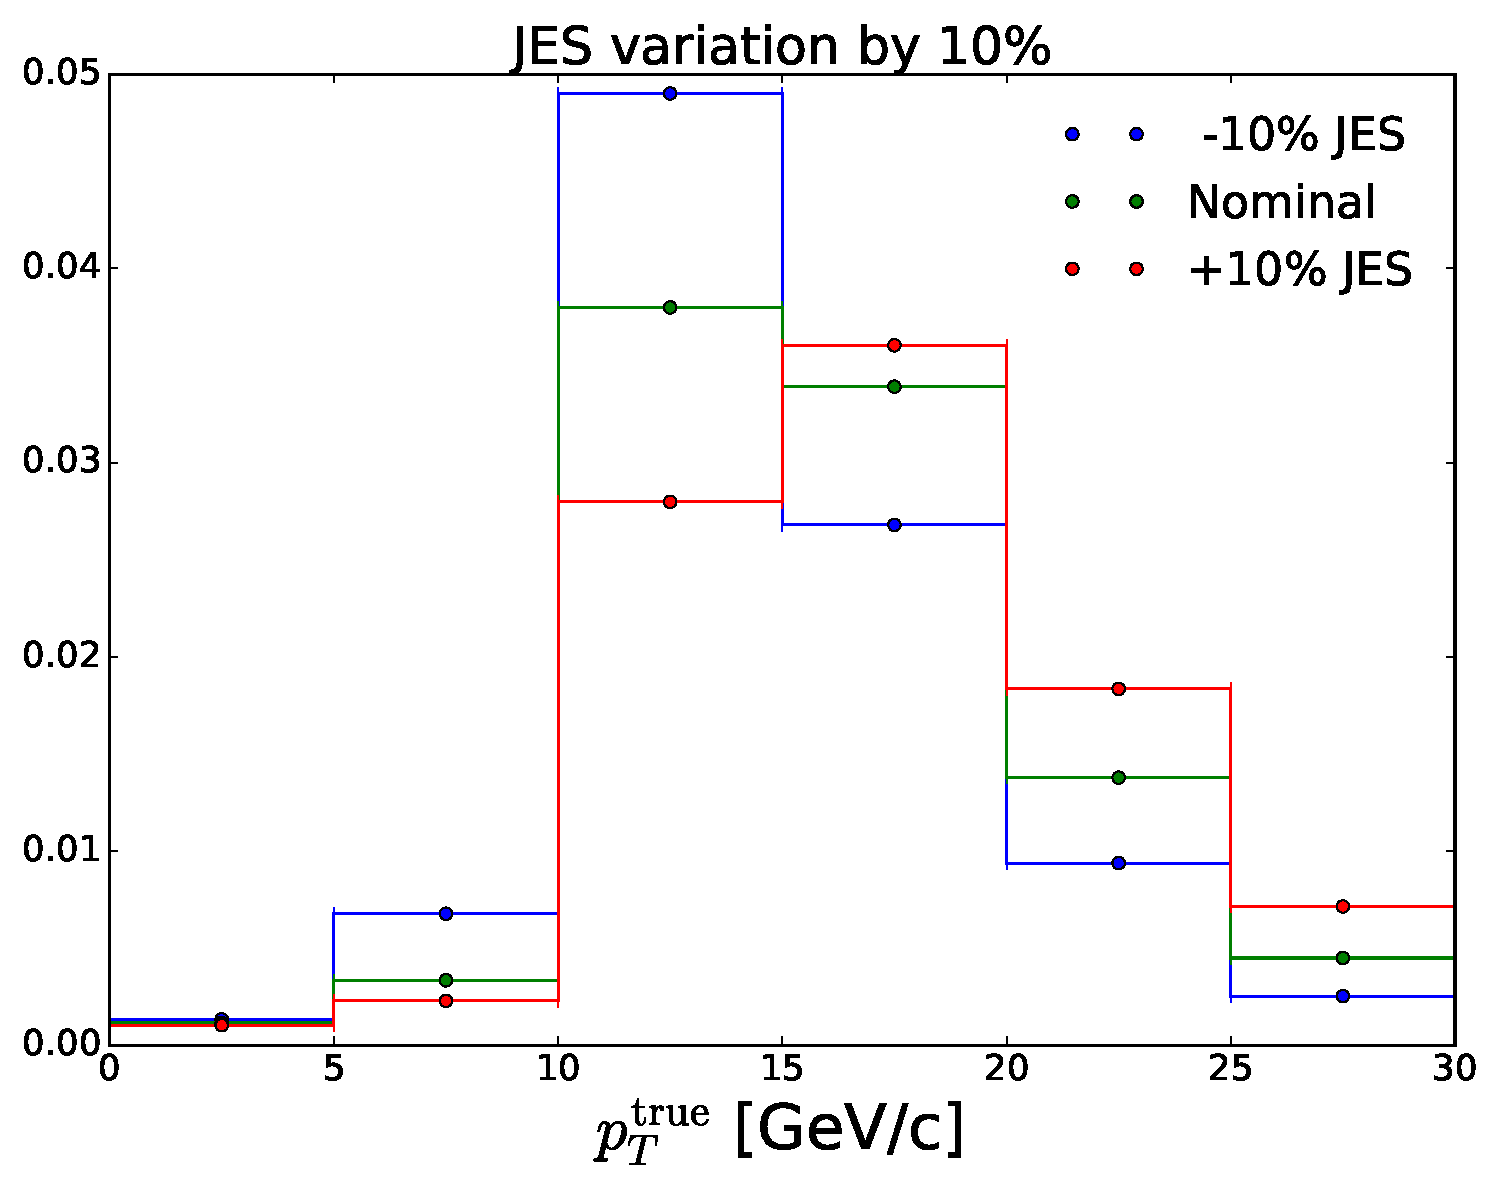
\includegraphics[width=0.5\textwidth]{EfficiencyAppendix/JES_variation.pdf}
%	\caption{}
%	\label{fig:JES_variation}
%\end{figure}
%\subsection{In-situ jet energy scale calibration}
%We reconstruct jets with only charged particles but we present results unfolded to the particle level. That is, we don't restrict the analysis to ``charged-only" jets or ``full-jets'' that include neutral energy, but rather all the energy. Obviously, this relies on the correct description of the absolute jet energy scale in MC simulations. The work in~\cite{JECNOTE} shows an {\it in situ} calibration based on $\gamma$--jet balance using a method first developed by CDF and D0 experiments at Tevatron and extensively used in the ATLAS and CMS experiments at the LHC. 
%The calibration results indicates that the jet energy scale is known to better than 4$\%$ for jets reconstructed with hybrid tracks (TPC+ITS). A cross-calibration from the jet-energy scale with ITS+TPC reconstruction to the ITS-standalone reconstruction yields a systematic uncertainty of $\pm10\%$. This validates our use of Monte Carlo simulations to correct (unfold) jets to the particle level. Moreover, we take into account this jet-energy scale uncertainty for our result in the Section~\ref{sec:systematics}


%\subsection{Check with p-A vs A-p}
%\FloatBarrier
%In this analysis, we have used the abbreviation "p-Pb" to refer to any asymmetric collision involving a proton and a lead nuclei. However only half of the dataset used in this analysis has the proton in the positive-eta direction and lead nuclei traveling in the negative-eta direction (pPb). The other half of the dataset used has the beams reversed (Pbp). Because $\Delta\eta$ is calculated as $\eta^{cluster}-\eta^{track}$, an asymmetry in $\eta^{track}$ resulting from the asymmetric collision system can potentially propagate as an asymmetry in our $\Delta\eta$ distributions. This section attempts to quantify any effects this may have on our final correlation function. 

%\begin{figure}
%\center
%\includegraphics[width=0.8\textwidth]{GammaHadron/p_Pb_Eta_Inclusive.png}
%\caption{$\Delta\eta$ projection of inclusive photon-hadron correlations for  %p-Pb collisions, where the lead-ion is traveling in the negative $\eta$ direction.}
%\label{fig:p-Pb_inclusive_eta}
%\end{figure}

%Figure \ref{fig:p-Pb_inclusive_eta} shows the $\Delta\eta$ projection of inclusive $\gamma$-hadron correlations in p-Pb collisions. While a very gradual slope can be seen in some $z_T$ bins, almost all points with the same absolute value of $\Delta\eta$ agree within uncertainties in each $z_T$ bin.

%\begin{figure}
%\center
%\includegraphics[width=0.8\textwidth]{GammaHadron/Pb_p_Eta_Inclusive.png}
%\caption{$\Delta\eta$ projection of inclusive photon-hadron correlations for  Pb-p collisions, where the lead-ion is traveling in the positive $\eta$ direction.}
%\label{fig:Pb-p_inclusive_eta}
%\end{figure}

%Figure \ref{fig:Pb-p_inclusive_eta} shows the $\Delta\eta$ projection for Pb-p collisions. The gradual slope from figure \ref{fig:p-Pb_inclusive_eta} is reversed, as expected. However, once again almost all points with the same magnitude agree within uncertainties in each $z_T$ bin.

%Thus, the hadron and jet measurements have no strong sensitivity to the rapidity shift at the pseudorapidity dependent variation of the underlying event within the statistical and systematic uncertainties of the measurement. Similar conclusion was reached in charged-jet measurement cross-section reported in Ref~\cite{Adam:2015hoa}.
%\item Shower shape selection:\\
%We quantify the uncertainty of our shower-shape selection by %performing independent analyses using the traditional $\lambdasquare$, $\emax$ and the deep-neural network approach. We use the corresponding measurement of purity for each case. The full difference of the final results is taken as a systematic uncertainty. We assume that this systematic uncertainty is uniformly distributed and quote a 1$\sigma$ that is scaled by $1/\sqrt{12}$. 
%\item Jet energy scale \\
%Given that the jet energy scale measurement is dictated by the tracking performance, for which we estimated a systematic uncertainty in the 5--10\% in Section~\ref{sec:tracking}, we conservatively estimate the systematic uncertainty on the jet energy scale to be $\pm$10$\%$. 

%We evaluate the systematic uncertainty due to jet-energy scale mismodelling in the simulation by varying the true jet~\pt by $\pm10\%$, which directly impacts the jet unfolding shown in Ref.~\ref{sec:jetunfolding}. This results in about 20--30$\%$ relative uncertainty on the jet yield, depending on the jet $\pt$.


%\item Unfolding: \\
%We estimate the systematic uncertainties associated with the unfolding procedure that we show in Section~\ref{sec:unfolding} by comparing the results obtained using different method. 
%\item UE-subtraction:\\
%As a conservative estimate, we take half the UE-subtraction estimated from the event mixing technique as our systematic uncertainty. This has a 5$\%$ effect on the yield in the 10--15 \GeVc and is negligible for higher $\pt$
